\chapter{Resultados e Discussão}
\label{cap:resultados}

\section{Análise Exploratória dos Dados}
\label{cap:resultados:sec:analise_exploratoria}

Foram identificados 814 hotéis distribuídos em todo o território nacional, desde hotéis de grandes redes e com disponibilidade de reservas do tipo \emph{All Inclusive} até hotéis pouco conhecidos com menos de 10 avaliações na plataforma.

Dessa lista temos como destaque os seguintes números:

Estados com a maior quantidade de hotéis
\begin{itemize}
	\item RJ: 71
	\item SP: 67
	\item PA: 62
	\item MG: 61
	\item RR/PI/MS: 60
\end{itemize}

Estados com a maior quantidade de avaliações

\begin{itemize}
	\item RJ: 231947 (4,22 com 71 hotéis)
	\item SP: 169586 (4,21 com 67 hotéis)
	\item BA: 107716 (4,34 com 22 hotéis)
	\item MG: 107067 (4,35 com 61 hotéis)
	\item PB: 68188 (4,36 com 54 hotéis)
\end{itemize}

Média da classificação dos hotéis por Estado

\begin{itemize}
	\item RS: 4,70 com 9493 avaliações no total (2 hotéis)
	\item AL: 4,64 com 33345 avaliações no total (8 hotéis)
	\item AC: 4,60 com 1696 avaliações no total (1 hotel)
	\item AM: 4,53 com 45509 avaliações no total (46 hotéis)
	\item SC: 4,50 com 32621 avaliações no total (7 hotéis)
\end{itemize}

Após aplicar o primeiro critério definido para a seleção da lista de hotéis, temos então uma lista com um grupo de 15 hotéis dentre os disponíveis, e após o filtro da região temos então 11. Também foram adicionados manualmente a lista outros 2 hotéis que atendiam os critérios hotéis que não foram listados nas consultas à \textit{API}.

A lista composta de 13 hotéis todos localizados na região nordeste do Brasil e com a disponibilidade de pacotes \emph{All Inclusive}, conforme tabela~\ref{table:lista_hoteis}, é valido notar que todos os hotéis da lista no momento da escolha possuíam uma avaliação na plataforma do \textit{Google Maps} com nota igual ou superior a 4.20 e são todos hotéis apontados pela plataforma como sendo hotéis de classificação de 4 ou 5 estrelas.

\begin{table}[]
	\begin{tabular}{|p{5cm}|l|r|r|l|r|}
		\hline
		\textbf{Nome}                                 & \textbf{Estado} & \textbf{Nota} & \textbf{Estrelas} & \textbf{Região} & \textbf{Quantidade} \\\hline
		Cana Brava All Inclusive Resort               & BA              & 4.60          & 4                 & NORDESTE        & 10987               \\\hline
		Grand Oca Maragogi                            & AL              & 4.30          & 5                 & NORDESTE        & 4613                \\\hline
		Hotel Marsol Beach Resort                     & RN              & 4.20          & 4                 & NORDESTE        & 3269                \\\hline
		Hotel Vila Galé - Touros                      & RN              & 4.60          & 5                 & NORDESTE        & 5619                \\\hline
		Hotel Vila Galé - Marés                       & BA              & 4.50          & 5                 & NORDESTE        & 8516                \\\hline
		Hotel Vila Galé: Eco Resort - Cabo            & PE              & 4.50          & 5                 & NORDESTE        & 5370                \\\hline
		Iberostar Bahia                               & BA              & 4.70          & 5                 & NORDESTE        & 16109               \\\hline
		La Torre Resort All Inclusive                 & BA              & 4.70          & 4                 & NORDESTE        & 6140                \\\hline
		Makai Resort Aracaju - All Inclusive          & SE              & 4.30          & 4                 & NORDESTE        & 5276                \\\hline
		Nauticomar Resort All Inclusive \& Beach Club & BA              & 4.30          & 4                 & NORDESTE        & 4258                \\\hline
		Salinas Maceió All Inclusive Resort           & AL              & 4.70          & 4                 & NORDESTE        & 4663                \\\hline
		Salinas Maragogi All Inclusive Resort         & AL              & 4.80          & 5                 & NORDESTE        & 7111                \\\hline
		Transamerica Comandatuba                      & BA              & 4.80          & 4                 & NORDESTE        & 3179                \\\hline
	\end{tabular}%
	\caption{Lista de hotéis e número de avalições}
	\label{table:lista_hoteis}
\end{table}

\begin{table}[]
	\centering
	\begin{tabular}{|l|l|}
		\hline
		\textbf{Ano} & \textbf{Quantidade} \\\hline
		2023         & 11925               \\
		2022         & 16364               \\
		2021         & 8104                \\
		2020         & 12489               \\
		2019         & 18963               \\
		2018         & 12625               \\
		2017         & 4426                \\
		2016         & 940                 \\
		2015         & 247                 \\
		2014         & 106                 \\
		2013         & 88                  \\
		2011         & 5                   \\
		2012         & 9                   \\
		\hline
	\end{tabular}%
	\caption{Quantidade de avaliações obtidas por ano}
	\label{table:review_per_year}
\end{table}

Considerando todas as avaliações obtidas podemos observar na tabela~\ref{table:review_per_year} que temos uma discrepância na quantidade e é perceptível a divisão no período de 2017/2018.
E dessa forma foi definido que serão utilizadas avaliações posteriores a 2018. Resultando um código conforme abaixo:

\lstinputlisting[language=Python,caption=Filtros aplicados ao dataset de avalições]{extras/code/review_filter.py}

Considerando todas as avaliações obtidas, temos:

\begin{itemize}
	\item 80470(93.25\%) enviadas depois de 2017 e 5821(6.75\%) enviadas em 2017, ou antes
	\item 56893(65.93\%) com texto e 3 ou mais caracteres, 29386(34.05\%) sem texto e 12(0.01\%) avaliações com 1 ou 2 caracteres
	\item 4184(4.85\%) avaliações traduzidas
\end{itemize}

Agora estamos considerando apenas avaliações que serão utilizadas na analise, a distribuição das notas atribuídas individualmente a cada avaliação pode ser consultada na Figura \ref{img:dist_review_rating}. É fácil notar que a grande maioria das avaliações registradas, mais especificamente 38347 (77,91\%), possui a maior nota atribuída, de valor 5, o que nos leva a acreditar que em grande parte das avaliações o sentimento geral que deve ser identificado será positivo.

\begin{figure}
	\centering
	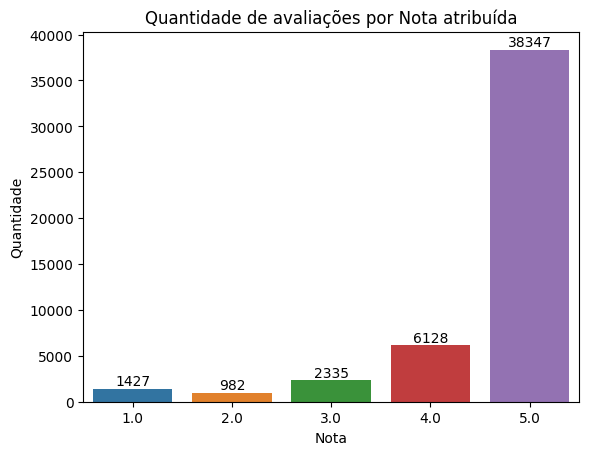
\includegraphics[width=0.75\textwidth]{figs/exploratoria/quantidade_avaliacao_nota_atribuida.png}
	\caption{Quantidade de avaliações por nota atribuida}
	\label{img:dist_review_rating}
\end{figure}

% possivel referencia? https://riull.ull.es/xmlui/handle/915/26220
Este comportamento de distribuição desigual das notas ainda é perceptível também quando olhamos para as avaliações agrupadas por ano de submissão, como pode-se notar na Figura \ref{img:dist_review_rating_per_year}. Podemos também observar na Figura \ref{img:dist_review_rating_per_year} a evolução em quantidade numérica durante o tempo, podendo notar uma quebra de tendência no crescimento pós 2019, nos anos de 2020 e 2021, provavelmente causado pelo confinamento decorrente da COVID-19 \cite{Guardia2022} e já pós flexibilização do confinamento, 2022, visualizamos um aumento expressivo no número de avaliações, levando ainda em consideração que temos apenas 6 meses de avaliação em 2023 então possivelmente seguiremos com a tendencia de aumento de número de avaliações ano após ano provavelmente 2023 será o ano com maior número de avaliações.

Com a Figura \ref{img:relplot_ano_rating} podemos notar que a variação da nota atribuída tende a diminuir conforme o tempo passa, pois a quantidade de notas maiores é cresce de forma desproporcional se comparado com as avaliações com notas baixas, como observado na Figura \ref{img:dist_review_rating_per_year}.

\begin{figure}
	\centering
	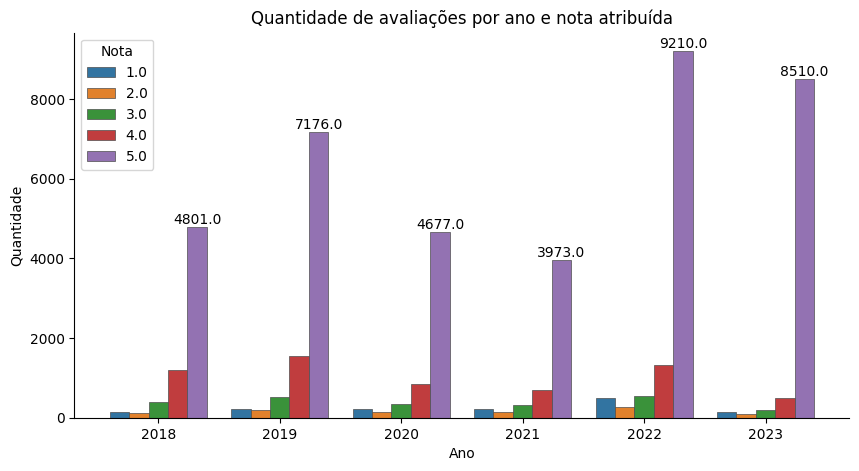
\includegraphics[width=1\textwidth]{figs/exploratoria/quantidade_avaliacao_nota_atribuida_ano.png}
	\caption{Quantidade de avaliações por ano e nota atribuída}
	\label{img:dist_review_rating_per_year}
\end{figure}

\begin{figure}
	\centering
	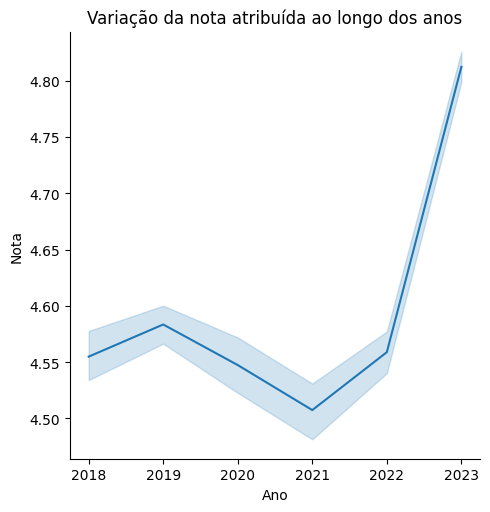
\includegraphics[width=0.70\textwidth]{figs/exploratoria/relplot_ano_rating.png}
	\caption{Variação da nota atribuída ao longo dos anos}
	\label{img:relplot_ano_rating}
\end{figure}

\begin{figure}
	\centering
	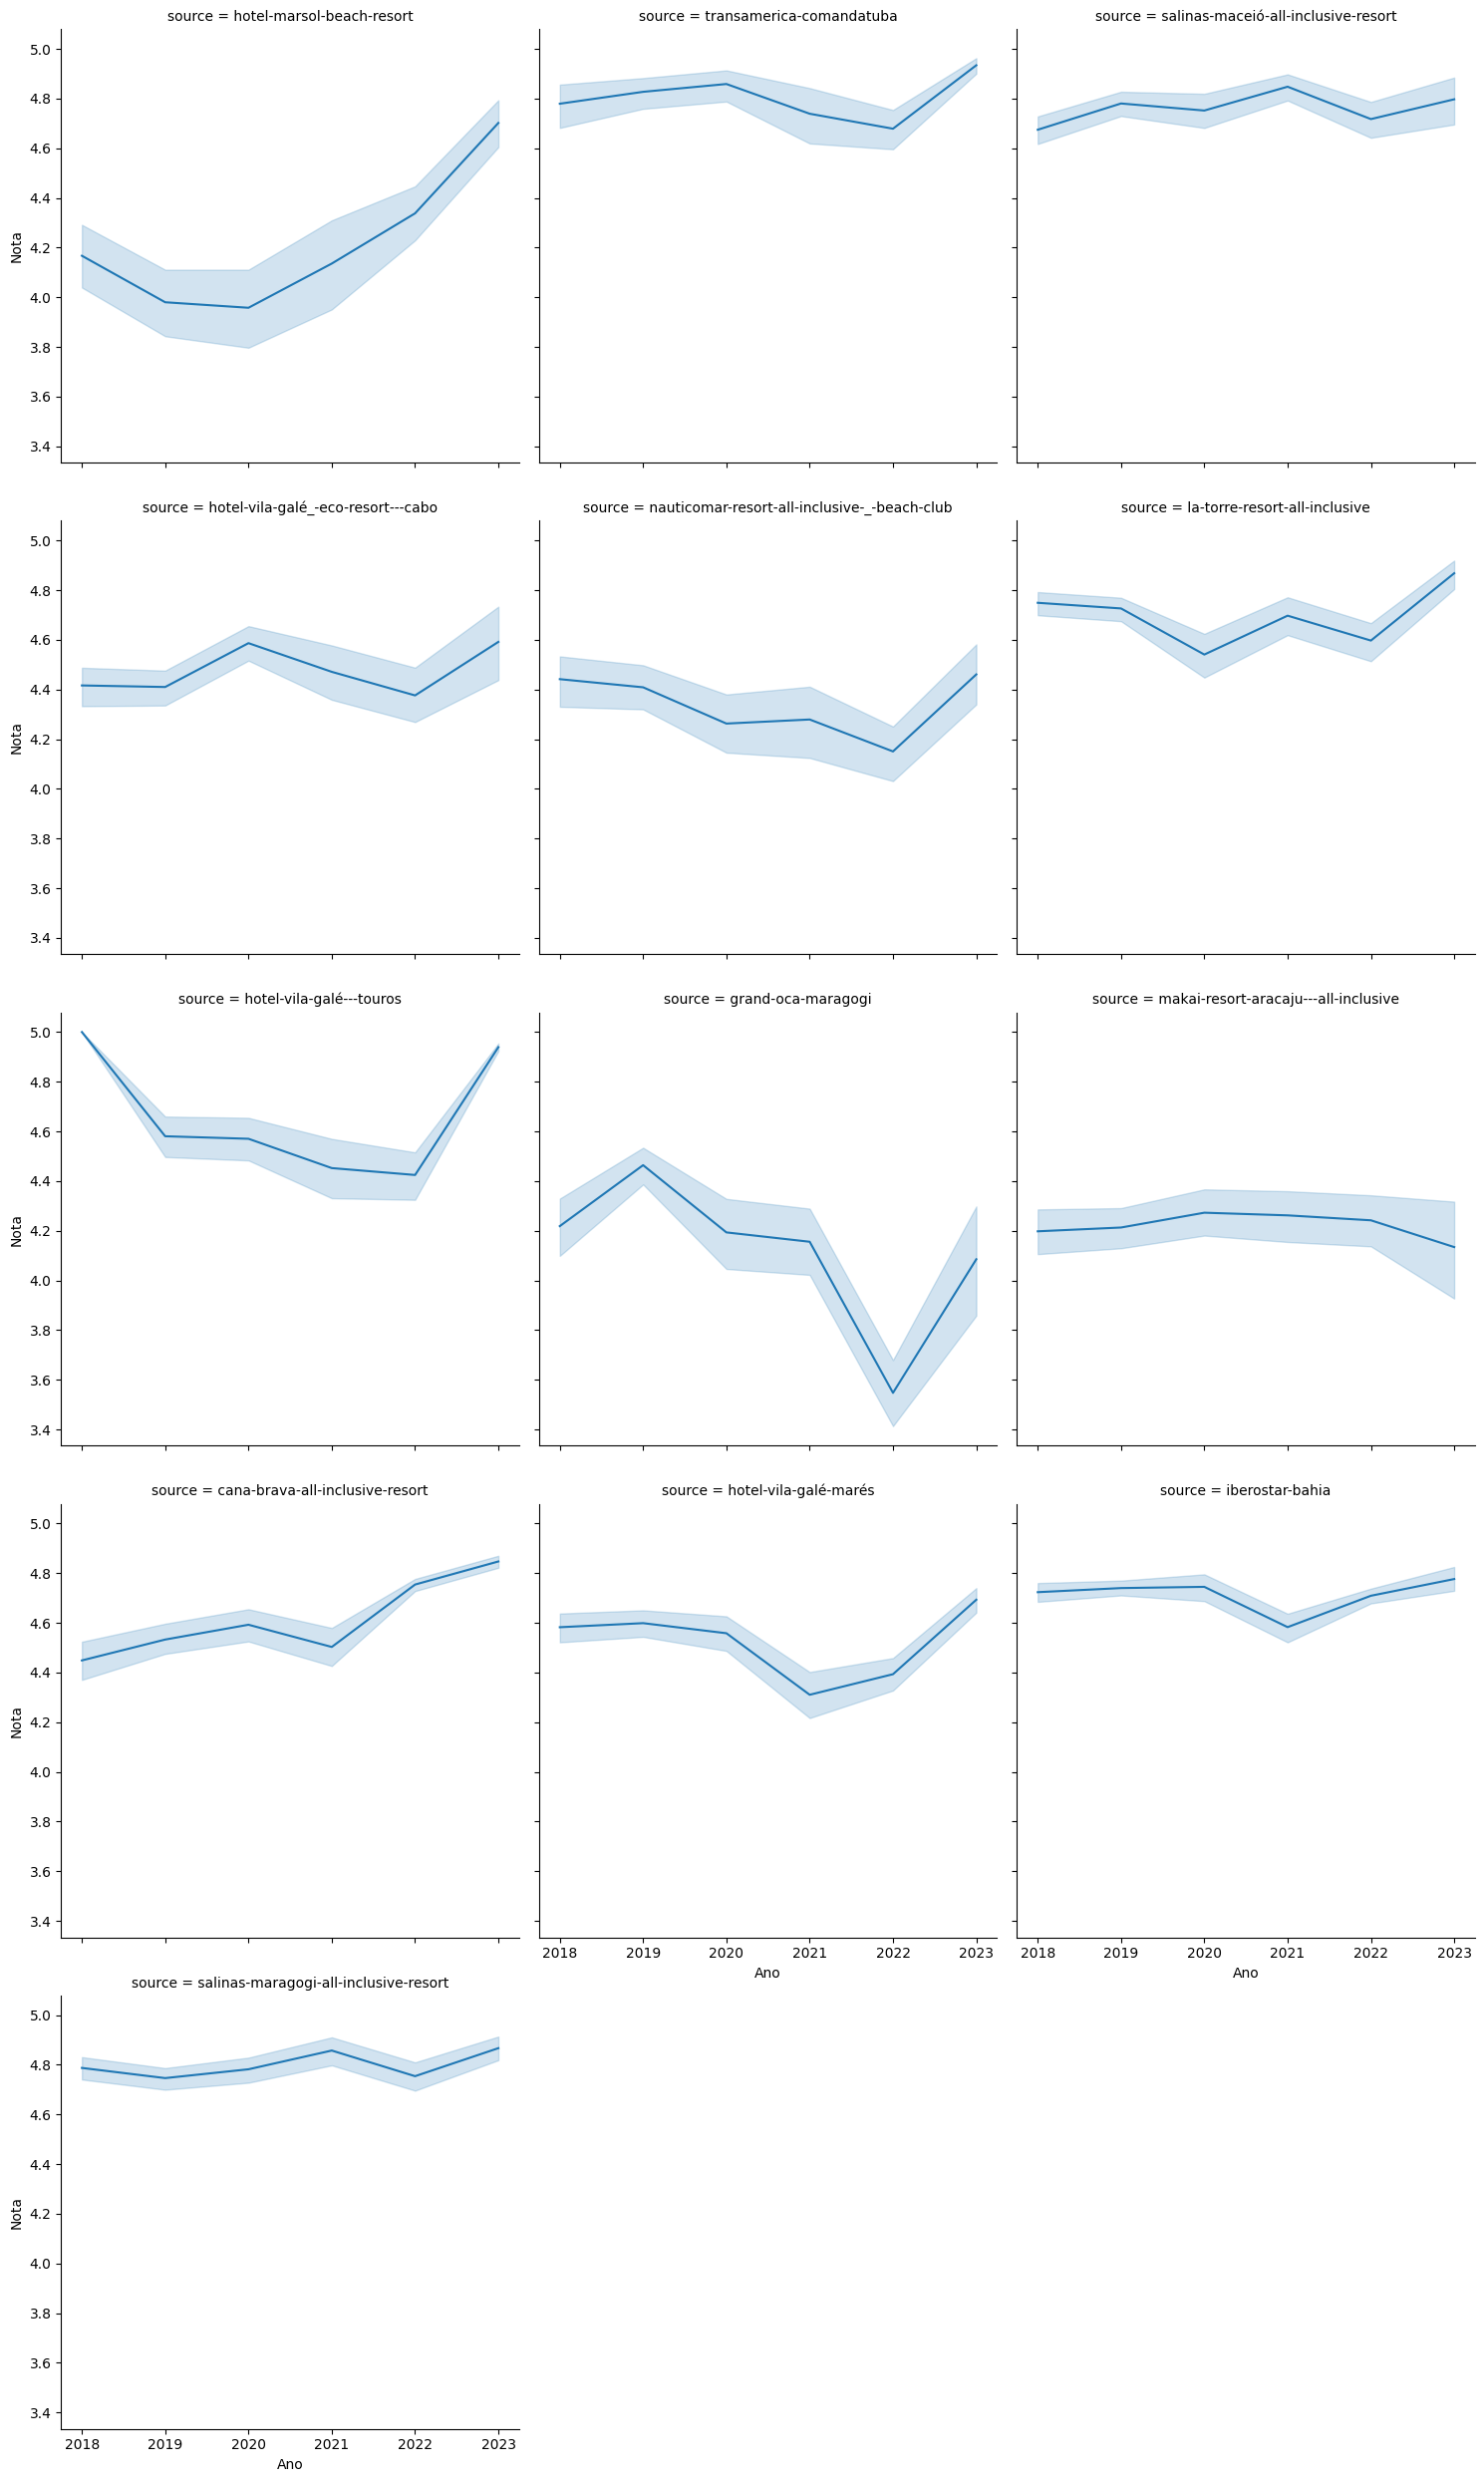
\includegraphics[width=1\textwidth]{figs/exploratoria/relplot_ano_rating_source.png}
	\caption{Variação da nota atribuída ao longo dos anos por hotel}
	\label{img:relplot_ano_rating_source}
\end{figure}

\begin{table}[]
	\centering
	\begin{tabular}{|p{5cm}|l|l|l|l|}
		\hline
		\textbf{Hotel}                                      &
		\textbf{Não vazio}                                  &
		\textbf{Com texto}                                  &
		\textbf{Traduzido}                                  &
		\textbf{Públicos em +2017}                            \\
		\hline
		\textbf{Cana Brava All Inclusive Resort}            &
		8583                                                &
		8581                                                &
		141                                                 &
		10656                                                 \\
		\hline
		\textbf{Grand Oca Maragogi}                         &
		2948                                                &
		2947                                                &
		542                                                 &
		4297                                                  \\
		\hline
		\textbf{Hotel Marsol Beach Resort}                  &
		2150                                                &
		2150                                                &
		162                                                 &
		3128                                                  \\
		\hline
		\textbf{Hotel Vila Galé - Touros}                   &
		4481                                                &
		4480                                                &
		111                                                 &
		5802                                                  \\
		\hline
		\textbf{Hotel Vila Galé - Marés}                    &
		5723                                                &
		5721                                                &
		315                                                 &
		7981                                                  \\
		\hline
		\textbf{Hotel Vila Galé Eco Resort - Cabo}          &
		3219                                                &
		3217                                                &
		183                                                 &
		4934                                                  \\
		\hline
		\textbf{Iberostar Bahia}                            &
		10587                                               &
		10586                                               &
		1464                                                &
		14848                                                 \\
		\hline
		\textbf{La Torre Resort - All Inclusive}            &
		3847                                                &
		3847                                                &
		496                                                 &
		5722                                                  \\
		\hline
		\textbf{Makai Resort Aracaju - All Inclusive}       &
		3180                                                &
		3180                                                &
		84                                                  &
		4917                                                  \\
		\hline
		\textbf{Nauticomar Resort All Inclusive Beach Club} &
		2630                                                &
		2628                                                &
		228                                                 &
		3938                                                  \\
		\hline
		\textbf{Salinas Maceió All Inclusive Resort}        &
		2836                                                &
		2836                                                &
		168                                                 &
		4497                                                  \\
		\hline
		\textbf{Salinas Maragogi All Inclusive Resort}      &
		4572                                                &
		4572                                                &
		203                                                 &
		6700                                                  \\
		\hline
		\textbf{Transamerica Comandatuba}                   &
		2149                                                &
		2148                                                &
		87                                                  &
		3050                                                  \\ \hline
	\end{tabular}
	\caption{Quantidade de avaliações em cada filtro pro hotél}
	\label{table:qtd_review_filtro}
\end{table}

Com os dados tratados agora possuímos a nova coluna \emph{mes\_ano\_avaliacao}, na Figura \ref{img:dist_ano_mes_avaliacao}, nota-se um comportamento estranho com a ausência de diversos meses por ano, durante o período de 2011 até 2021 temos o registro de apenas avaliações no mês 7, este comportamento é devido ao formato de data relativa utilizada pelo \textit{Google Maps} ao expor suas avaliações, não foi possível identificar uma forma de adquirir o tempo definitivo de quando a avaliação foi publicada, por este motivo ao utilizar a data relativa e para as avaliações mais antigas conseguimos apenas identificar o ano no qual a avaliação foi publicada, as avaliações com menos de um ano de diferença da data de recuperação utilizando este \textit{script} poderiam ser utilizadas em uma analise mais detalhada em relação ao período, porém esta não foi a estrategia escolhida e optaremos por restringir a análise de maneira em que as avaliações serão agrupadas em períodos anuais, representando assim o ano de publicação de cada avaliação.

\begin{figure}
	\centering
	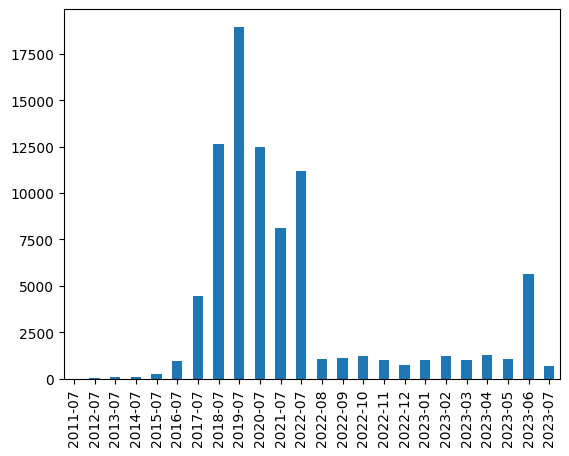
\includegraphics[width=0.75\textwidth]{figs/exploratoria/distribuicao_ano_mes_avaliacao.png}
	\caption{Distribuição do número de avaliação por mês e ano}
	\label{img:dist_ano_mes_avaliacao}
\end{figure}

\begin{table}[]
	\centering
	\begin{tabular}{|c|crrrrr|}
		\hline
		\multicolumn{1}{|c|}{\multirow{2}{*}{\textbf{Estado}}} &
		\multicolumn{2}{c|}{\textbf{analisar}}                 &
		\multicolumn{3}{c|}{\textbf{nota}}                     &
		\multicolumn{1}{c|}{\textbf{estrelas}}                                                                            \\ \cline{2-7}
		\multicolumn{1}{|l|}{}                                 &
		\multicolumn{1}{c}{\textbf{rotulo}}                    &
		\multicolumn{1}{c|}{\textbf{quantidade}}               &
		\multicolumn{1}{c}{\textbf{média}}                     &
		\multicolumn{1}{c}{\textbf{min}}                       &
		\multicolumn{1}{c|}{\textbf{max}}                      &
		\multicolumn{1}{c|}{\textbf{média}}                                                                               \\ \hline
		\multirow{2}{*}{\textbf{AL}}                           & \textbf{False} & 8106  & 4.623896 & 4.3 & 4.8 & 4.735998 \\
		                                                       & \textbf{True}  & 8668  & 4.643205 & 4.3 & 4.8 & 4.706853 \\ \hline
		\multirow{2}{*}{\textbf{BA}}                           & \textbf{False} & 20970 & 4.617740 & 4.3 & 4.8 & 4.542680 \\
		                                                       & \textbf{True}  & 28727 & 4.613016 & 4.3 & 4.8 & 4.467017 \\ \hline
		\multirow{2}{*}{\textbf{PE}}                           & \textbf{False} & 2645  & 4.500000 & 4.5 & 4.5 & 5.000000 \\
		                                                       & \textbf{True}  & 2746  & 4.500000 & 4.5 & 4.5 & 5.000000 \\ \hline
		\multirow{2}{*}{\textbf{RN}}                           & \textbf{False} & 2903  & 4.397451 & 4.2 & 4.6 & 4.493627 \\
		                                                       & \textbf{True}  & 6232  & 4.480424 & 4.2 & 4.6 & 4.701059 \\ \hline
		\multirow{2}{*}{\textbf{SE}}                           & \textbf{False} & 2448  & 4.300000 & 4.3 & 4.3 & 4.000000 \\
		                                                       & \textbf{True}  & 2846  & 4.300000 & 4.3 & 4.3 & 4.000000 \\ \hline
	\end{tabular}\caption{Quantidade de avaliações por estado e por rotulo -- indicando o que será e o que não será analisado}
	\label{table:distribuicao_review_por_estado}
\end{table}

E dentre todas as avaliações obtidas após aplicar o filtro de período utilizaremos para a análise o total de 49219(57.04\%) e 37072(42.96\%) foram ignoradas. Assim as avaliações que foram consideradas estão então distribuídas conforme \ref{table:distribuicao_review_per_year}.

\begin{table}[]
	\centering
	\begin{tabular}{|l|l|}
		\hline
		\textbf{Ano} & \textbf{Quantidade} \\\hline
		2023         & 9444                \\
		2022         & 11866               \\
		2021         & 5350                \\
		2020         & 6236                \\
		2019         & 9645                \\
		2018         & 6678                \\
		\hline
	\end{tabular}
	\caption{Quantidade de avaliações por ano após filtro}
	\label{table:distribuicao_review_per_year}
\end{table}

% TODO

\begin{table}[]
	\centering
	\begin{tabular}{|c|c|r|r|}
		\hline
		\multicolumn{1}{|r|}{\textbf{Hotel}}                                    &
		\multicolumn{1}{r|}{\textbf{Analisar?}}                                 &
		\textbf{Quantidade}                                                     &
		\textbf{\%}                                                               \\ \hline
		\multirow{2}{*}{\textbf{Cana Brava All Inclusive Resort}}               &
		False                                                                   &
		3028                                                                    &
		27.16                                                                     \\ \cline{2-4}
		                                                                        &
		True                                                                    &
		8119                                                                    &
		72.84                                                                     \\ \hline
		\multirow{2}{*}{\textbf{Grand Oca Maragogi}}                            &
		False                                                                   &
		2427                                                                    &
		52.34                                                                     \\ \cline{2-4}
		                                                                        &
		True                                                                    &
		2210                                                                    &
		47.66                                                                     \\ \hline
		\multirow{2}{*}{\textbf{Hotel Marsol Beach Resort}}                     &
		False                                                                   &
		1470                                                                    &
		44.10                                                                     \\ \cline{2-4}
		                                                                        &
		True                                                                    &
		1863                                                                    &
		55.90                                                                     \\ \hline
		\multirow{2}{*}{\textbf{Hotel Vila Galé - Touros}}                      &
		False                                                                   &
		1433                                                                    &
		24.70                                                                     \\ \cline{2-4}
		                                                                        &
		True                                                                    &
		4369                                                                    &
		75.30                                                                     \\ \hline
		\multirow{2}{*}{\textbf{Hotel Vila Galé - Marés}}                       &
		False                                                                   &
		3550                                                                    &
		41.36                                                                     \\ \cline{2-4}
		                                                                        &
		True                                                                    &
		5033                                                                    &
		58.64                                                                     \\ \hline
		\multirow{2}{*}{\textbf{Hotel Vila Galé: Eco Resort - Cabo}}            &
		False                                                                   &
		2645                                                                    &
		49.06                                                                     \\ \cline{2-4}
		                                                                        &
		True                                                                    &
		2746                                                                    &
		50.94                                                                     \\ \hline
		\multirow{2}{*}{\textbf{Iberostar Bahia}}                               &
		False                                                                   &
		7830                                                                    &
		48.29                                                                     \\ \cline{2-4}
		                                                                        &
		True                                                                    &
		8383                                                                    &
		51.71                                                                     \\ \hline
		\multirow{2}{*}{\textbf{La Torre Resort All Inclusive}}                 &
		False                                                                   &
		3164                                                                    &
		50.84                                                                     \\ \cline{2-4}
		                                                                        &
		True                                                                    &
		3060                                                                    &
		49.16                                                                     \\ \hline
		\multirow{2}{*}{\textbf{Makai Resort Aracaju - All Inclusive}}          &
		False                                                                   &
		2448                                                                    &
		46.24                                                                     \\ \cline{2-4}
		                                                                        &
		True                                                                    &
		2846                                                                    &
		53.76                                                                     \\ \hline
		\multirow{2}{*}{\textbf{Nauticomar Resort All Inclusive \& Beach Club}} &
		False                                                                   &
		2104                                                                    &
		49.03                                                                     \\ \cline{2-4}
		                                                                        &
		True                                                                    &
		2187                                                                    &
		50.97                                                                     \\ \hline
		\multirow{2}{*}{\textbf{Salinas Maceió All Inclusive Resort}}           &
		False                                                                   &
		2140                                                                    &
		45.72                                                                     \\ \cline{2-4}
		                                                                        &
		True                                                                    &
		2541                                                                    &
		54.28                                                                     \\ \hline
		\multirow{2}{*}{\textbf{Salinas Maragogi All Inclusive Resort}}         &
		False                                                                   &
		3539                                                                    &
		47.46                                                                     \\ \cline{2-4}
		                                                                        &
		True                                                                    &
		3917                                                                    &
		52.54                                                                     \\ \hline
		\multirow{2}{*}{\textbf{Transamerica Comandatuba}}                      &
		False                                                                   &
		1294                                                                    &
		39.95                                                                     \\ \cline{2-4}
		                                                                        &
		True                                                                    &
		1945                                                                    &
		60.05                                                                     \\ \hline
	\end{tabular}
	\caption{Lista de quantidade de avaliações analisadas e descartadas por hotel}
	\label{tab:lista_review_hoteis}
\end{table}

Após devido tratamento das avaliações conseguimos obter as nuvens de palavras considerando todas as palavras na Figura \ref{img:wordcloud_geral}, onde podemos notar como alguns dos destaques quarto, piscina, praia, restaurante, como sendo as palavras com maior frequência nas avaliações.


Já considerando a nuvem de palavras filtrando apenas por adjetivos teremos então na Figura \ref{img:wordcloud_adjetivos} que tem como alguns dos destaques palavras como sensacional, excelente, especial, local, top, ótimo, nota.

E por ultimo observamos a nuvem de palavras levando em consideração apenas os substantivos na Figura \ref{img:wordcloud_substantivos}, que como destaque podemos citar funcionário, piscina, quarto, praia.

Uma outra forma de analise é o agrupamento de tokens em unigramas na Figura \ref{img:unigramas}, bigramas na Figura \ref{img:bigramas} e os trigramas na Figura \ref{img:trigramas} presentes em todas as avaliações. dessa forma temos exatamente a classificação de franquênia dos tokens no corpus de estudo.

Entre os unigramas \ref{img:unigramas} temos uma lista com alguns dos tokens mais frequentes, alguns chegando a passar a contagem de utilização de mais de 10.000 vezes, como é o caso de lugar, sendo seguindo ainda que próximo por comida, excelente e atendimento, este ultimo com uma frequência próximo de 8500 vezes. Ainda em relação aos unigramas também podemos levar em consideração a sua frequência com a evolução do tempo em \ref{img:rank_unigramas}, e algo com grande destaque é a palavra lugar que está entre o top 10 entre todo o período da analise, flutuando entre as cinco primeiras posições, tio é um unigrama que merece atenção, por não ter aparecido na nuvem de palavras de unigramas, porém se faz presente no ranking se observarmos individualmente os anos ele aparece em décimo lugar no ano de 2022, indícios de uma possível atração local bem conhecida, substituindo então o unigrama 'praia', que se fazia presente no ranking até 2021 na nona colocação.

Considerando os bigramas \ref{img:bigramas} a frequência diminui consideravelmente, pois aqui temos que a ordem importa e dessa forma o mais frequente fica próximo de 1700 vezes, sendo composto pela dupla 'lugar' e 'maravilhoso', seguido pelo segundo colocado, bem próximo de 1400 vezes, sendo 'comida' e 'boa', onde podemos observar a grande frequência de palavras positivas, por conta dos adjetivo positivos.

Para destaque entre os trigramas \ref{img:trigramas} a frequência diminui ainda mais e como destaque temos um que supera a contagem de 250 vezes, sendo 'facilidade', 'deslocamento' e 'pe', o que nos indica que existe pelo menos um hotel que possui uma boa localização para que seja possível se deslocar até uma atração popular do local à pé, seguido de 'atendimento', 'nota' e '10' que indica que para as pessoas que avaliaram o atendimento da rede de hotéis ainda é algo importante e que deve ser levado em consideração caso a rede tenha interesse em ter ou manter um conceito positivo entre seus cliente.


\begin{figure}
	\centering
	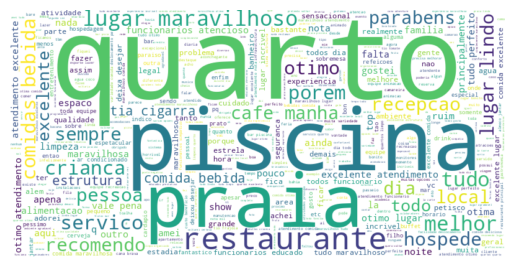
\includegraphics[width=1\textwidth]{figs/exploratoria/wordcloud_geral.png}
	\caption{Wordcloud sem stop words}
	\label{img:wordcloud_geral}
\end{figure}


\begin{figure}
	\centering
	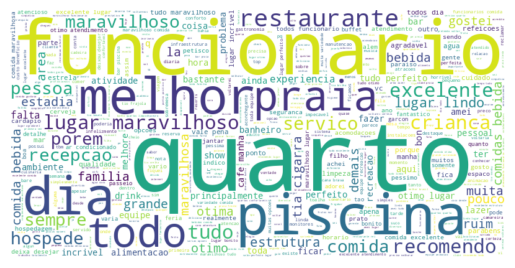
\includegraphics[width=1\textwidth]{figs/exploratoria/wordcloud_substantivos.png}
	\caption{Wordcloud de substantivos}
	\label{img:wordcloud_substantivos}
\end{figure}

\begin{figure}
	\centering
	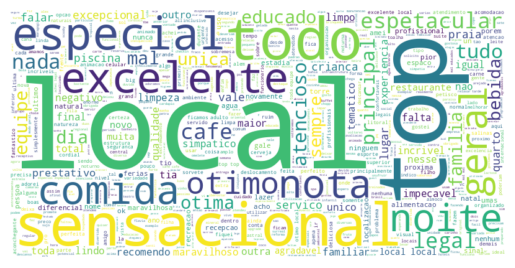
\includegraphics[width=1\textwidth]{figs/exploratoria/wordcloud_adjetivos.png}
	\caption{Wordcloud de Adjetivos}
	\label{img:wordcloud_adjetivos}
\end{figure}

\begin{figure}
	\centering
	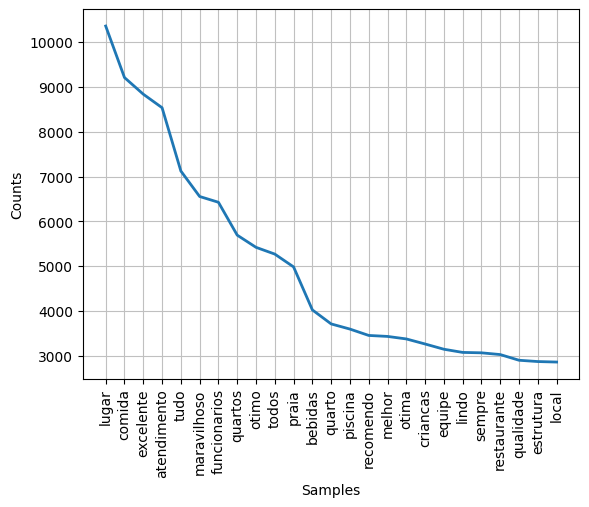
\includegraphics[width=1\textwidth]{figs/exploratoria/unigramas.png}
	\caption{Unigramas}
	\label{img:unigramas}
\end{figure}

\begin{figure}
	\centering
	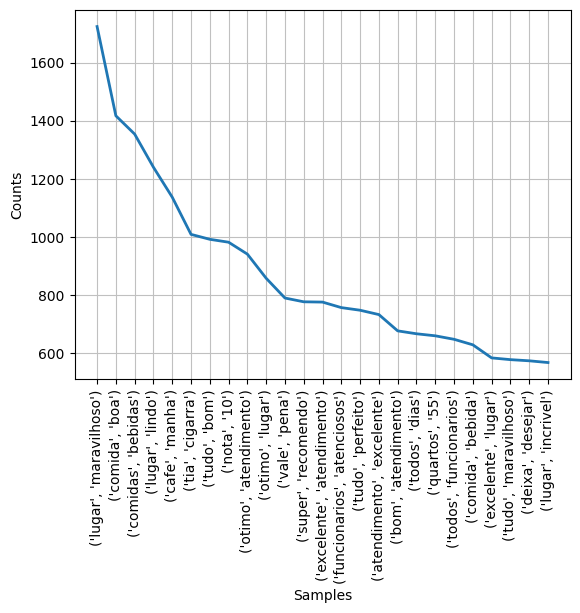
\includegraphics[width=1\textwidth]{figs/exploratoria/bigramas.png}
	\caption{Bigramas}
	\label{img:bigramas}
\end{figure}

\begin{figure}
	\centering
	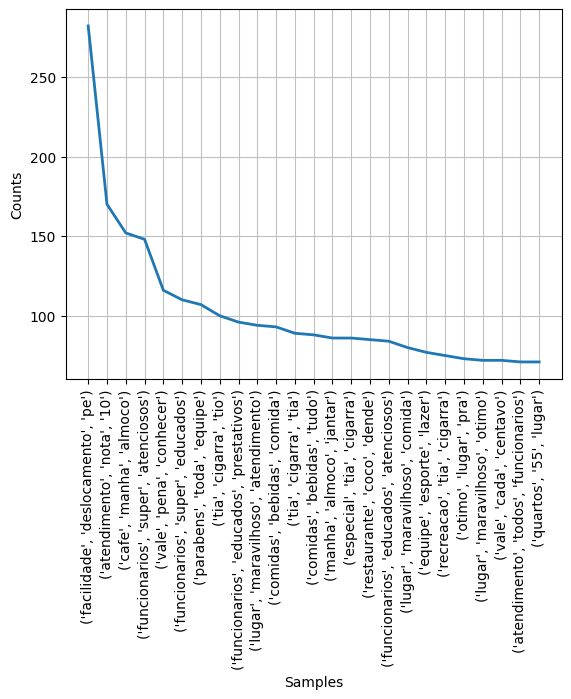
\includegraphics[width=1\textwidth]{figs/exploratoria/trigramas.png}
	\caption{Trigramas}
	\label{img:trigramas}
\end{figure}


%TODO ajustar tamanho, ta estranho
\begin{figure}
	\centering
	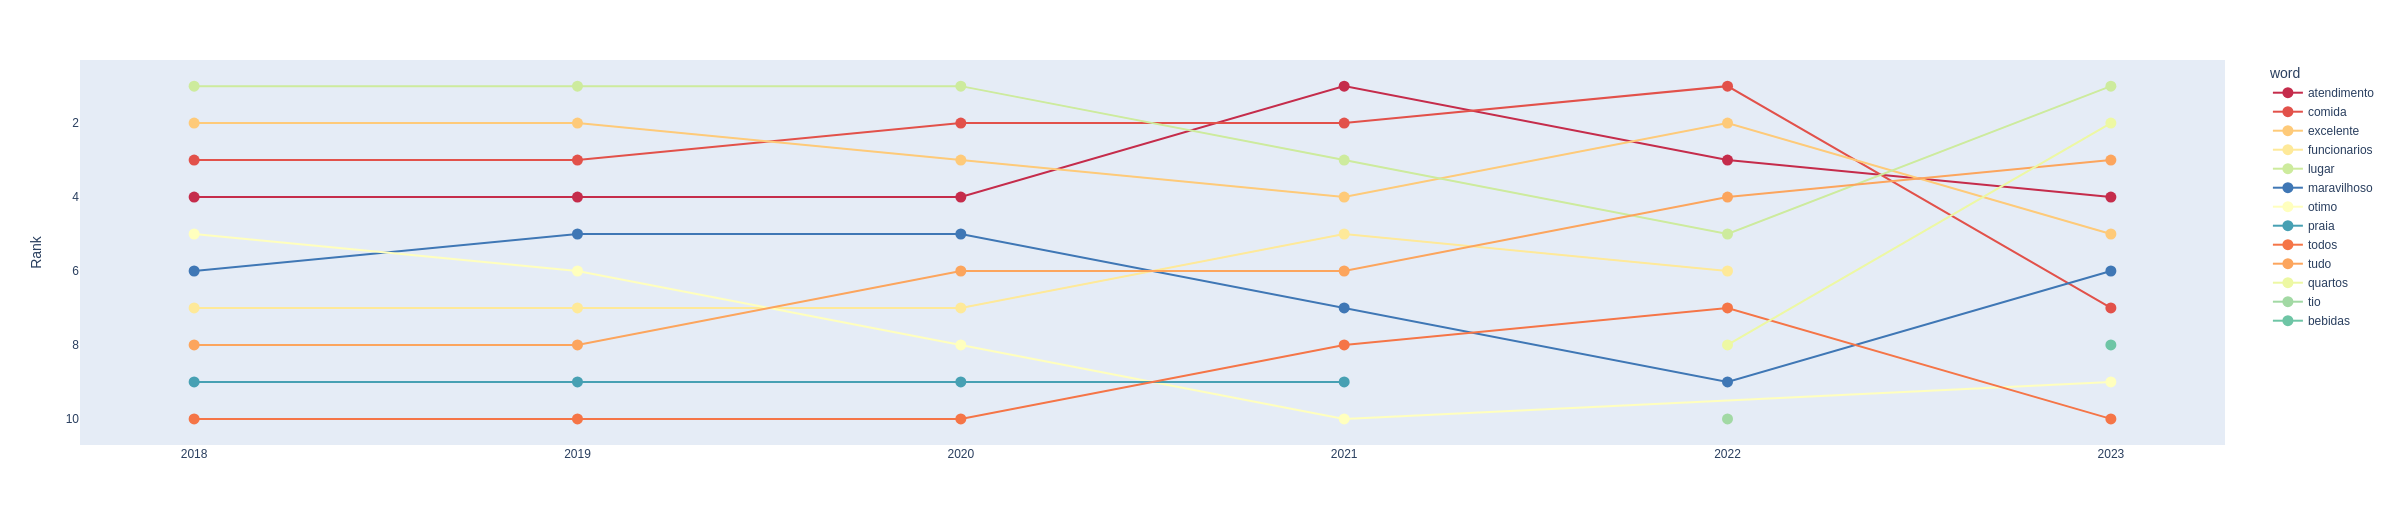
\includegraphics[width=.7\textwidth]{figs/exploratoria/ranking_unigramas_por_ano.png}
	\caption{Ranking de unigramas por ano}
	\label{img:rank_unigramas}
\end{figure}

\section{Análise de Sentimentos Temporal}
\label{cap:resultados:sec:analise_sentimento}

\subsection[BERT]{BERT}
\label{sec:resultados:subsec:bert}

O tempo de execução médio, após 5 execuções cada, para que a analise de todo o corpos fosse realizada, o seguinte:

\begin{itemize}
	\item philschmid/distilbert-base-multilingual-cased-sentiment: 3min e 37s
	\item lxyuan/distilbert-base-multilingual-cased-sentiments-student: 3min e 36s
	\item citizenlab/twitter-xlm-roberta-base-sentiment-finetunned: 6min e 54s
	\item cardiffnlp/twitter-xlm-roberta-base-sentiment: 6min e 44s
	\item ramonmedeiro1/bertimbau-products-reviews-pt-br: 6min e 59s
\end{itemize}


% \subsection[Grandes Modelos de Linguagem]{Grandes Modelos de Linguagem}
% \label{sec:resultados:subsec:bert}
% E dentre todas as avaliações obtidas utilizaremos para a analise o total de 49219(57.04\%) e 37072(42.96\%) foram ignoradas

\subsection{Vicuna}

\subsection{GPT 3.5}

Utilizando o modelo GPT 3.5 para realizar a tarefa de analise de sentimentos do conteúdo textual das avaliações obtemos a distribuição conforme Figura \ref{img:gpt_pizza_distribuicao}, onde 84.77\% das avaliações, ou seja, 41721 avaliações foram classificadas como tendo um sentimento positivo, isso representa um número próximo das avaliações que receberam como nota 4 ou 5, 6128 e 38347 avaliações respectivamente, porém fica fácil notar na Figura \ref{img:gpt_sentimento_nota} que mesmo a grande maioria das avaliações com essa nota atribuída ainda existem avaliações com sentimentos diferentes

\begin{figure}
	\centering
	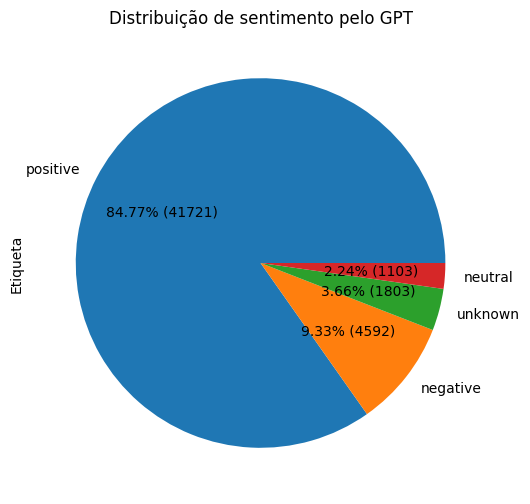
\includegraphics[width=1\textwidth]{figs/gpt/distribuicao_pizza.png}
	\caption{Distribuição do sentimento das avaliações}
	\label{img:gpt_pizza_distribuicao}
\end{figure}

\begin{figure}
	\centering
	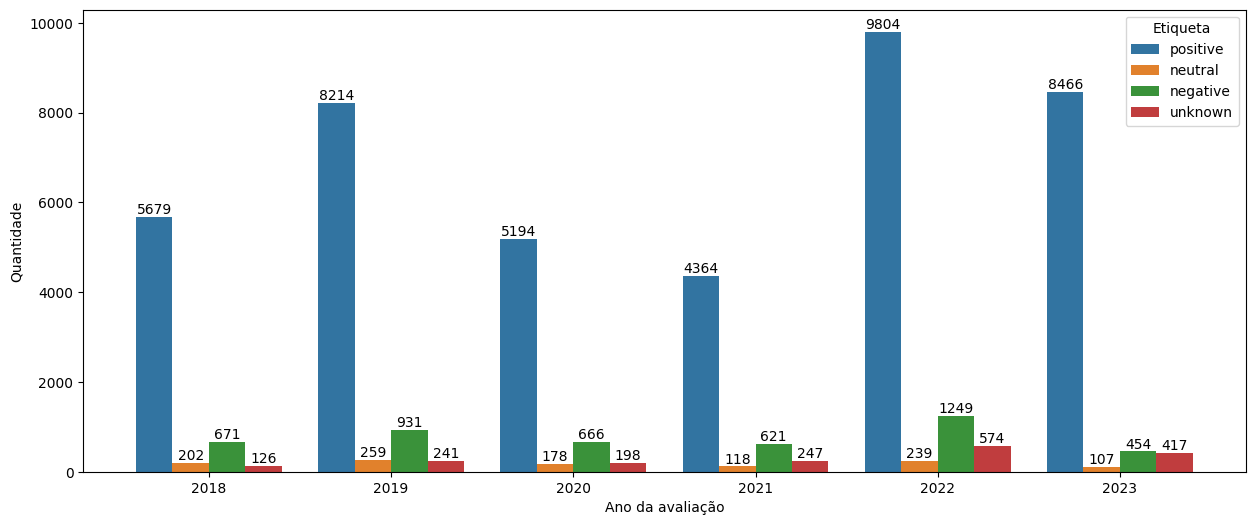
\includegraphics[width=1\textwidth]{figs/gpt/sentimento_ano.png}
	\caption{Sentimento das avaliações por ano}
	\label{img:gpt_sentimento_ano}
\end{figure}

\begin{figure}
	\centering
	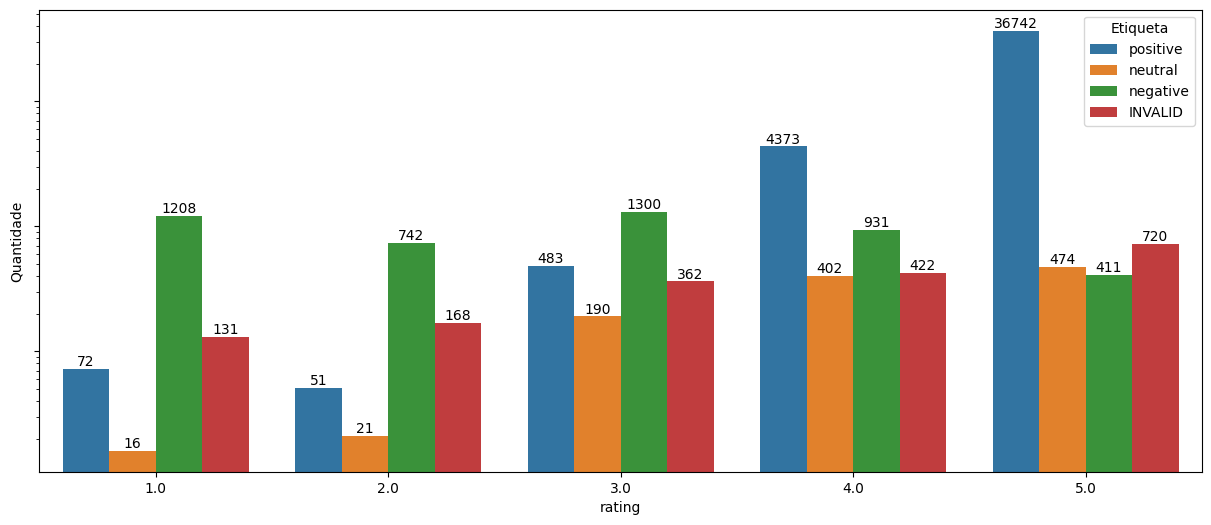
\includegraphics[width=1\textwidth]{figs/gpt/sentimento_nota.png}
	\caption{Sentimento das avaliações por nota}
	\label{img:gpt_sentimento_nota}
\end{figure}


\subsection{OpenChat}


% sentimento bert

% sentimento gpt

% sentimento temporal

% outros LLMs

% bert vs GPT

% inconsistencias? revalidaçoes?
